%----------------------------------------------------------------------------------------
%	KOPPEN EN BIJLAGE
%----------------------------------------------------------------------------------------

\section{An Overview of Pipelining}									%Het titel van het hoofdstuk - plaats deze alleen wanneer deze samenvatting over de eerst sectie gaat.
\subsection{Pipelining}
							%De titel van de sectie / paragraaf uit het boek en de naam van de samenvatter.
												%Hanteer bij voorkeur dezelfde sectienummers als in het boek!
\begin{wrapfigure}{r}{0pt}
\attachfile{hoofdstuk.tex}									%Bijvoegen van het oorspronkelijke .tex bestand, pas bestandsnaam waar nodig aan.
\end{wrapfigure}

%----------------------------------------------------------------------------------------
%	SAMENVATTING
%----------------------------------------------------------------------------------------

	Pipelining is een implementatie techniek waarbij meerdere instructies elkaar overlappen tijdens het uitvoeren. Het paradoxale aan pipelining is dat je er een enkele instructie niet sneller mee maakt. De reden dat voor meerdere instructies pipelining sneller is is dat het instructies simultaan verwerkt waardoor het geheel eerder klaar is.
	\begin{quote}
		{\small\texttt{Bij MIPS bestaan instructies meestal uit 5 stappen
			\begin{enumerate}
				\item Instructie uit het geheugen ophalen
				\item Register uitlezen tijdens het decoderen van de instructie
				\item Operatie uitvoeren of adres berekenen
				\item Operator gebruiken in het geheugen
				\item Schrijf het resultaat in het geheugen
			\end{enumerate}
		}}
	\end{quote}
	De versnelling door pipelining kan je in onderstaande formule weergeven, uitgaande van ideale omstandigheden$$Time between instructions_{pipelined} = \frac{Time between instructions_{nonpipelined}}{Number of pipe stages}$$
	Onder ideale omstandigheden en met een grote hoeveelheid instructies is de versnelling doormiddel van pipelining even groot als het aantal stappen in de pipeline.
	\subsection{Designing Instruction Sets for Pipelining}
	Door alle instrucies de zelfde lengte te maken, zoals bij MIPS, is het veel makkelijker om in de eerste stap in de pipeline de instructies op te halen en ze in de tweede stap te decoderen.\\
	Ook een beperkt aantal instructie formats met gelijkende indeling zorgt er voor dat het makkelijker is om te pipelinen.\\
	Doordat geheugen operatoren alleen load en store operaties voorkomen in MIPS kan in stap 3 het geheugen adres berekent worden en daarna in stap 4 aangesproken worden.
	\subsection{Pipeline Hazards}
	\subsubsection{Structural Hazard}
	Wanneer de hardware de combinatie van instructies die je in dezelfde clock cycle wilt uitvoeren niet ondersteunt
	\subsubsection{Data hazard}
	Wanneer een geplande instructie niet uitgevoerd kan worden in de goede clock cycle omdat de data die nodig is nog niet beschikbaar is.
	\subsubsection*{Forwarding}
	Een manier om een data hazard te voorkomen door de ontbrekende data uit de interne buffers te halen in plaats van uit de voor de programmeur zichtbare registers of geheugens.
	\subsubsection{Load-Use Data Hazard}
	Een specifieke data hazard waarbij de data die geladen wordt door een load instructie nog niet beschikbaar gekomen is wanneer het bij een andere instructie nodig is.
	\subsubsection*{Pipeline Stall}
	Een vertraging gebruikt om een hazard te voorkomen.
	\subsubsection{Control Hazard}
	Wanneer de goede instructie niet in de goede clock cycle kan  worden uitgevoerd omdat de opgehaalde instructie niet de nodige instructie is, vanwege een branch.\\
	\texttt{Zie pagina 282 voor voorbeeld.}
	\subsubsection*{Branch Prediction}
	Een methode om een control hazard te verhelpen door een aanname te nemen van welke branch het gaat worden inplaats van te wachten op een definitieve uitkomst.
	\subsection{Pipelined Datapath and Control}
	Het datapath is opgedeeld in 5 delen:
	\begin{enumerate}
		\item IF: Instruction fetch
		\item ID: Instruction decode and register file read
		\item EX: Execution or address calculation
		\item MEM: Data memory access
		\item WB: Write back
	\end{enumerate}
	In het onderstaande figuur staat het met de onderdelen weergegeven.\\
	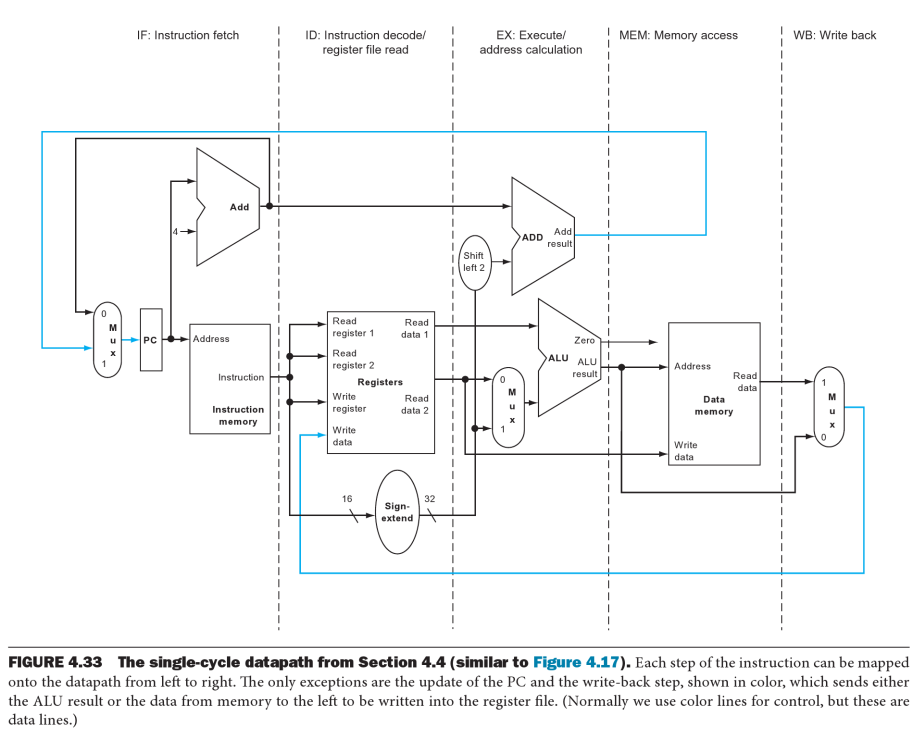
\includegraphics[scale=0.6]{Fig4_33.png}\\
	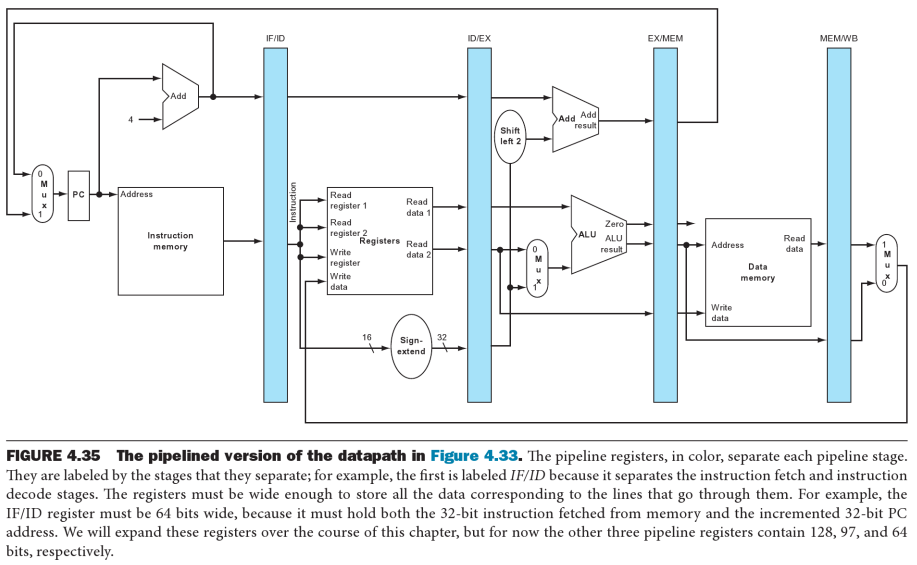
\includegraphics[scale=0.6]{Fig4_35.png}\\
	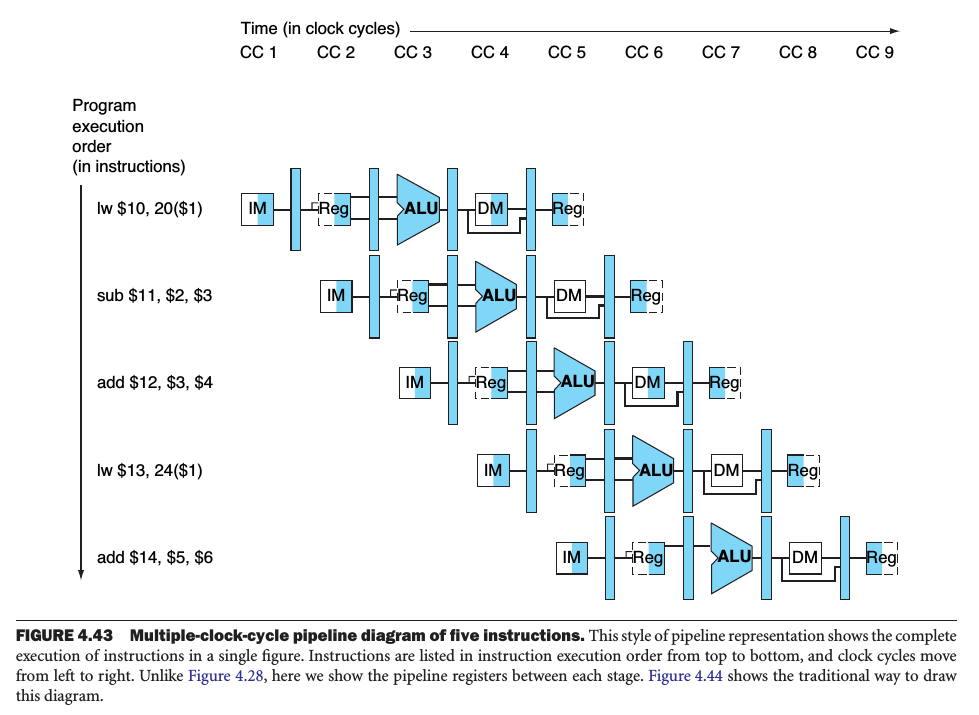
\includegraphics[scale=0.6]{Fig4_43.png}\\
	\pagebreak
	\subsubsection*{Pipelined Control}
	Hieronder staat hoe de controlle signalen ingebouwd worden.\\
	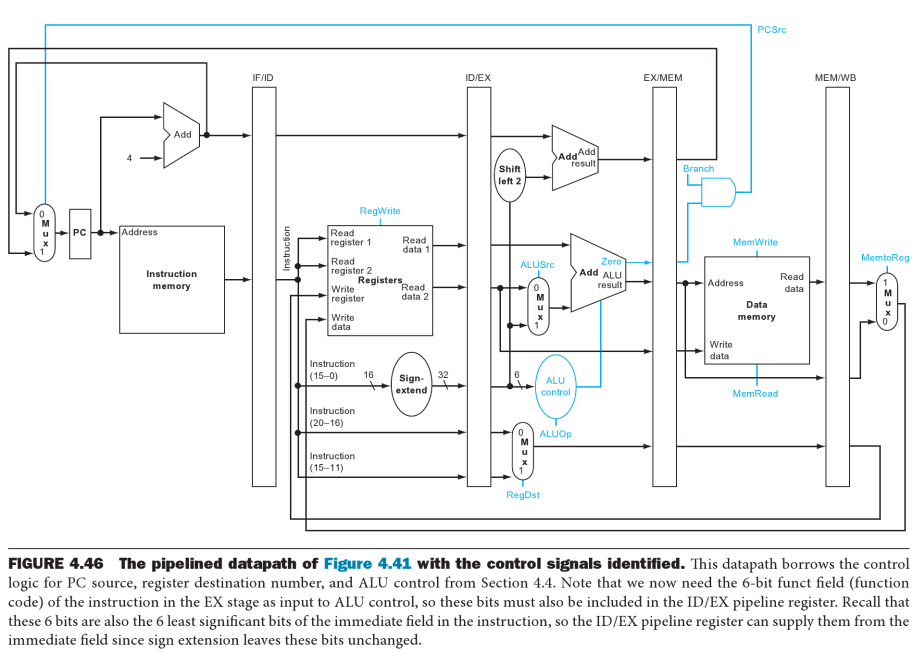
\includegraphics[scale=0.6]{Fig4_46.png}\\
	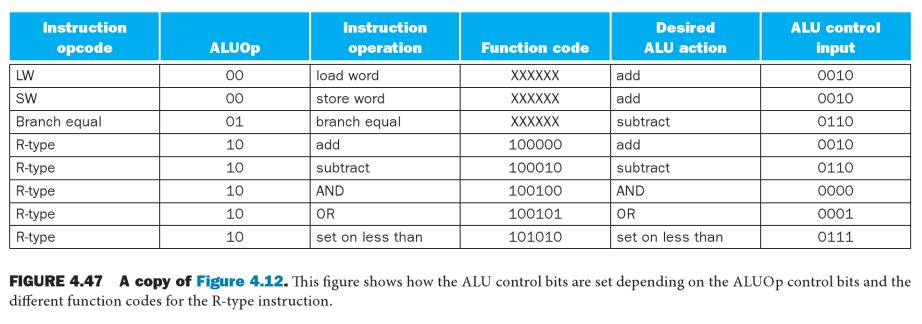
\includegraphics[scale=0.6]{Fig4_47.png}\\
	De controle signalen kunnen in vijf groepen verdeeld worden:
	\begin{enumerate}
		\item Instruction fetch
		\item Instruction decode/Register file read
		\item Execution/Address calculation
		\item Memory access
		\item Write back
	\end{enumerate}
	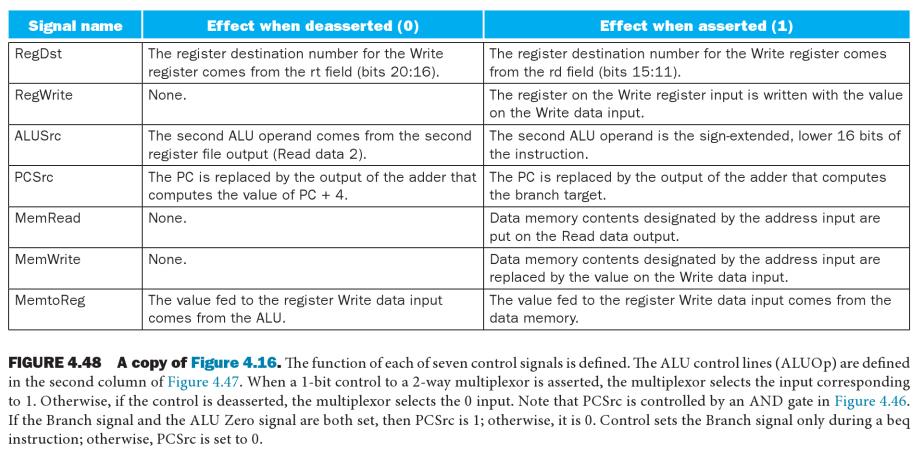
\includegraphics[scale=0.6]{Fig4_48.png}\\
	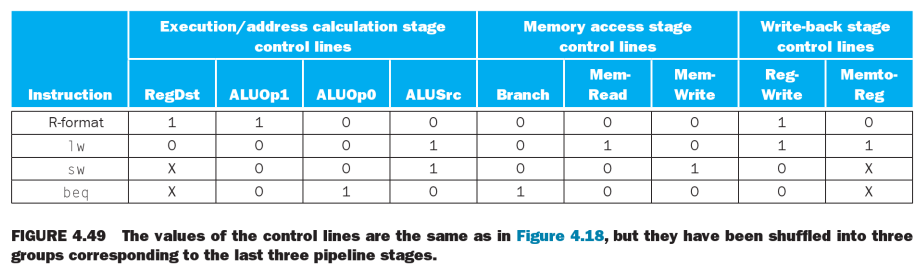
\includegraphics[scale=0.6]{Fig4_49.png}\\